\section{Introduction}
Android applications have become a staple of many people's everyday mobile computing user experience.  As of the first quarter of 2017 Android possessed 85\% of the mobile phone market \cite{chau_2017}.  The need for complete and thorough testing capabilities of Android applications has never been greater.  

A common problem with automated mobile software testing is testing mobile applications when the state of the device change is not being considered despite often catastrophic affects of device state on an application.  It is more expensive to not test device states against application states at all.  Testing the different states of an application has been enhanced with tools such as Espresso and Robotium \cite{optimusinformationinc2016}.  Since the state of an application can be easily saved and the state of a device can be easily changed programmatically, a solution that automatically tests application states with different device states is of great value.  For applications being used in different device states, such as a "mapping" applications used outside of network range or medical applications using sensors for monitoring functions, application to device state testing becomes an extremely important issue.  Some of these issues can even be life safety critical.  Additionally, the innovative ways applications are used with new hardware is only increasing.  State testing of applications with new hardware devices is a critical area of research to ensure that applications can continue to operate well. 

In addition to state testing, there is a strong need for innovative approaches to testing context aware applications \cite{Luo:2017:TLT:3139486.3130945}.  A context aware application is an application that is able to detect information about the device's physical environment using instrumentation and then do something with that information.  

"The field of mobile specific, black-box testing, however, remains thin." \cite{paulovsky2017high}  That is the reasoning behind this endeavor to make easier testing tools that easily test the interaction of device states with applications states.  

We have developed a Mobile application called "TADS" (Test Application to Device State) that uses Espresso, an automated Android application testing tool, to test the Mobile application against multiple states and sub-states of the device \cite{366932}.  TADS is primarily concerned with identifying errors caused by changing device states and not as concerned with identifying why the state change caused a failure.

\section{Research Contributions}
This work demonstrates that a library for doing state testing of devices that can be run with espresso is highly beneficial and easy to make.  This research contributes a tool that can be used right now for anyone wanting to improve their test suites to include device state testing.. 

The second contribution this work makes is a very simple way for testing context-aware applications' handling of instrumentation state changes. The work done in \cite{Luo:2017:TLT:3139486.3130945} produces test data for context applications, this work tests the affect of changing the state of the instruments used by those applications.  A DSC can be easily generated that changes the states of the instruments that the context aware application uses in order to ensure changing instrumentation states will not cause a failure. 

The evaluation questions to be explored are the following.

RQ1: Can an easy to use method of testing device state against existing test suites be developed?

RQ2: Can device state interference be detected using a state testing method that can then be used by developers to respond to such device state interference? 

\section{Background}
As of the writing of this paper, there is not any research available about automatic device state testing.  In order to understand this project a few items must be known ahead of time.  

Espresso, an android testing application, has an excellent tool for testing Mobile application UI's \cite{nolan2015agile}.  The tool records what is happening at a code level while a user performs different actions using the UI.  This enables a working application to have a test automatically generated that can then be run at a later time which can be used to create a regression test suite.  This actually enables states of the application to be tested without having to use any form of state machines or modeling.  This tool called "Test Recorder" is foundational to TADS. 

"Android Debug Bridge, is a command-line utility included with Google's Android sdk. ADB can control your device over USB from a computer, copy files back and forth, install and un-install apps, run shell commands, and more." \cite{hoffman2017}  TADS relies heavily on the Android Device Bridge  ADB . The Adb allows scripts to be written adn run that dynamically change device states.


\section{Related Work}
There are several tools developed that can capture various information of an application and store said information for later tests.  These tools can be leveraged to create interesting app states instead of simple object states.  For instance Paulovsky et al. \cite{7962332} built a tool that automatically captures UI information as a user utilizes an application. 

The most similar work to TADS is called Barista by Fazzini et al. \cite{7927971}.  They made a tool that can store UI information and then auto generate oracles that then get scripted into an Espresso test script for later use as a test case.  This tool could be used to run test cases as the DSCs execute as the state instead of static properties being evaluated. This solution cannot evaluate device state; though, the researchers have added doing so to their future works section.   

Many others, such as \cite{7927971} have made tools for recording tests that can be later executed in ways that are platform independent which is a nice utility that we will not be concerned with in this work.  Others have made unit level state testing models such as MilaniFard el al. \cite{MilaniFard:2014:LET:2642937.2642991} in which the state of the application is tested by automatically building a model using a dynamic and static crawler and then running that created model against a verification algorithm.  G. Bai et al developed a way to use model testing to find security vulnerabilities \cite{7911333}.  Choi et al have used machine learning to find the states of an application that are probably of value to test that have not been tested and make a model of those states for testing \cite{Choi:2013:GGT:2544173.2509552}.


\section{Implementation}
The main purpose of this Application is to simplify testing of different device states with the application.  There are preloaded "device state changes" (DSCs) that can be used in a test suite to test the app states that are chosen for testing.  A DSC is a test case that starts with a device state then runs the test cases and then changes the Devices state.  The DSC then runs the tests again with the new state set.  A few examples of DSCs are: airplane mode off, run a test suite or test case, switch airplane mode to on, then re-run a test suite or test case.

The TADS solution is built on Microsoft Power Shell and written as Power Shell scripts.  Power Shell was decided on to enforce DRY and SOLID principles without the convolution of building an executable program that is compiled.  Additionally Powershell levereges the strength of the .NET runtime and libraries for easier implementation of complex algorithms.    

The solution is run by running a powershell script from the command line with parameters that are the name of your solution and tests that should be run.

Table 1 is a break down of the functions to be called by your command line or in a script that a developer would write to test their application how they deem necessary.  

There is a readme file that should be followed to get the testing environment set up for usage of the TADS solution.  The TADS solution can be downloaded at: \url{https://github.com/UCCS-CS5371-Fall2017/jsander7/tree/master/ProjectFiles} \\

\begin{figure}[t]
	\centering
	\caption[Public Interface]{Public Interface}
	\label{fig:table1}
	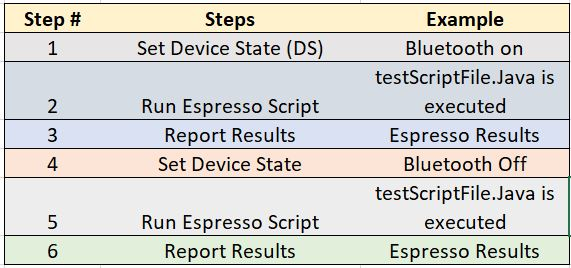
\includegraphics[width=1\linewidth]{table1}
\end{figure}

The implementation allows a user to call a function to test the following as is shown in Figure 1.  The user can run all of their test suites and all of the DSC's available, all tests and 1 DSC that is selected, 1 DSC and 1 test case in the suite, and all DSCs and 1 test case. The name of the application should be the whole app name starting with "com.". The public interface in Figure 1 is what novice programmers should use.   

All functions in the entire solution are available to be consumed by the user.  This is so that a programmer can build their own Powershell script out of the existing functions.  

Within the TADS solution there are three main files.  They are DSCs.psm1, TestSuiteCommands.psm1, and ADBCommands.psm1.  The DSCs file contains all of the DSCs which is comprised of calls to the TestSuiteCommands and ADBCommands.  The TestSuiteCommands file contains the public interface found in Figure 1 and the commands that run the test suites in Espresso.  The ADMCommands file is where the state change commands are located that use ADB to change the states of the device. 

\section{Evaluation}
This is gibberish because I still am unsure how to evaluate this project.  Lorem ipsum dolor sit amet, consectetur adipiscing elit. Quisque laoreet facilisis dolor sit amet iaculis. Sed in ante lacinia purus accumsan commodo. Sed ut purus ante. Integer sed dictum urna. Vivamus vehicula quam sed urna placerat, at egestas dui malesuada. Vestibulum lectus urna, congue at malesuada at, pellentesque in mauris. Duis quam turpis, euismod nec lobortis sit amet, pretium non felis. Donec interdum purus in mi lacinia, ornare egestas nibh varius. Etiam semper elementum dolor nec malesuada. Pellentesque vestibulum vehicula velit ut fermentum. Donec mi eros, consequat vitae feugiat eget, commodo feugiat sem. Duis ultricies, justo quis faucibus accumsan, erat nisi cursus mi, nec imperdiet justo leo id nulla. Nunc at sodales turpis.

Sed non sem ac odio varius efficitur eget quis dui. Fusce mattis eros non convallis molestie. Fusce at mi dictum, cursus mauris vel, interdum erat. Vivamus fermentum lectus tristique dui varius interdum vel at enim. Vestibulum nisl turpis, consequat at quam sed, vulputate suscipit lectus. Duis et placerat odio, sed sollicitudin mi. Cras eleifend vulputate fermentum. Class aptent taciti sociosqu ad litora torquent per conubia nostra, per inceptos himenaeos. Etiam efficitur ullamcorper tincidunt. Suspendisse augue enim, commodo ut felis ut, accumsan rutrum mi. Mauris varius ornare vulputate. Proin neque leo, pulvinar id varius vel, fringilla nec dolor. Duis facilisis maximus metus nec rutrum.

Aliquam rutrum dui ipsum, quis egestas ante dapibus a. Maecenas eleifend, elit non ullamcorper imperdiet, odio enim congue leo, nec consequat nibh magna eget mi. Nulla dignissim ipsum ac tortor molestie, sit amet pulvinar odio semper. Vestibulum lobortis velit nec enim finibus, et accumsan nisi porta. Phasellus tincidunt malesuada ultrices. Nunc a neque quis sem elementum semper vel eu arcu. Donec vitae varius lacus. Nullam id urna maximus, consectetur ligula a, faucibus massa.

Aenean egestas ut nisl quis vehicula. Duis euismod bibendum felis in porta. Ut ut nisl at felis aliquam lacinia id eget ipsum. Nunc auctor dictum aliquet. Praesent sed orci nunc. Quisque placerat enim quis egestas pellentesque. Vivamus egestas dui dolor. Pellentesque at lectus non mauris viverra pellentesque eget et leo. Pellentesque luctus felis id laoreet euismod. Vestibulum vel eros nec velit tincidunt pellentesque. Quisque vitae malesuada augue. Suspendisse et vestibulum nulla.

Aliquam volutpat felis interdum risus laoreet pulvinar vitae at purus. Donec mauris sapien, placerat quis euismod vel, hendrerit at metus. Suspendisse vitae odio sit amet orci viverra interdum eu ut urna. Morbi porta tincidunt odio, eleifend finibus urna pulvinar sed. Fusce egestas nulla sed dui imperdiet, tempor sagittis felis rhoncus. Mauris elementum sed ex eget sollicitudin. Nullam malesuada, sem non porttitor fringilla, risus diam mattis enim, ut sollicitudin magna sapien et sem. Vivamus tempus vel nibh non mattis.

\section{Future Research}
A future research opportunity would be to implement the TADS solution in a way that the state changes can be called easily within an Espresso script.  That would enable knowledgeable testers to correctly evaluate the affect of different state changes on their solutions at specific times during execution of the script.   

Another challenge is that commands do not exist for ADB to change proprietary device instrumentation states.  Figuring out how to instantiate different hardware devices from the command interface and easily implement new DSCs will prove extremely beneficial in making robust state testing of Android applications using proprietary instrumentation suchh as a portable Electrocardiograms.  

Barista \cite{7927971} provides a better script generation tool than Espresso.  Integrating TADS to run Barista could prove to be a valuable endeavor.  Also, being able to inject DSCs into Barista generated testing scripts will enhance the ability of Barista to catch bugs introduced by device state changes.  

We also hope to expand the instrumentation capabilities to include wearable devices such as Android watch or even google glass for state testing with apps running on those devices.

Another approach that could prove extremely beneficial is to evaluate the affect of these sttes and state changes on the efficiency of an application. One could create a way of capturing pertinent throughput data and run some form of an evaluative algorithm against that date thereby giving developers pertinent information on how to improve their application's efficiency by using some kind of brownout technique \cite{Klein:2014:BBM:2568225.2568227} or other viable solution when that device state is detected. 

The last future research we are considering at this time is to investigate how device state affects installs.  Installations can be affected by the state of different items running on a device and building a test script that installs an application and running that installation on devices with different states may prove valuable; though, some research into whether or not industry struggles with installations being affected by state would be an interesting approach.  

ADD table with dsc's and the name of them with a note in the caption stating more would be added if actually publishing.  


\section{Threats to Validity}
One serious threat to this work is that the automated test scripts built in Espresso can be affected by state changes \cite{7927971} which can cause a failure in the test due to the script's failure and not the application's.  This error will be revealed by the logging utility and corrections can be made a test design time.  

